% Section 6. Rewritten 2026-11-03 (branch docs/cep-grounded-draft) from src/optics/disambiguate.py and the rerun in
% docs/optics/rerun_results.md (scripts/rerun_paper_numbers.py). Claim changes: papers/cep/CLAIM_CHANGES.md.
\section{Front/back disambiguation with a single-component size prior}\label{sec:sizing}

\subsection{The front/back ambiguity and the size signal}\label{sec:ambiguity}

Circular-aperture defocus is symmetric in reciprocal object distance (\secref{sec:coc}): two depths with
$1/d_\mathrm{near} + 1/d_\mathrm{far} = 2/d_\mathrm{focus}$ produce the same blur, so a single image does not tell
whether a blurred object lies in front of or behind the focal plane~\citep{SellentFavaro2014}. The apparent size of a
crystal of physical width $w$, however, is monotone in $d_o$. With the pixel scale proportional to object distance,
$\Delta x(d_o) = \Delta x(d_\mathrm{focus})\, d_o / d_\mathrm{focus}$ (\secref{sec:thinlens}),
\begin{equation}\label{eq:spx}
s_\mathrm{px}(d_o) = \frac{w}{\Delta x(d_o)}, \qquad
\frac{s_\mathrm{px}(d_\mathrm{near})}{s_\mathrm{px}(d_\mathrm{far})} = \frac{d_\mathrm{far}}{d_\mathrm{near}},
\end{equation}
\begin{equation}\label{eq:ratio}
\frac{d_\mathrm{far}}{d_\mathrm{near}} - 1 \approx \frac{2\delta}{d_\mathrm{focus}} \quad
(\delta = d_\mathrm{focus} - d_\mathrm{near} \ll d_\mathrm{focus}).
\end{equation}
Equal blur with unequal apparent size is the signal a size prior can exploit. Its strength is set by $\delta$, that
is, by how far from focus the detector still finds crystals (\secref{sec:selectivity}).

\subsection{Homogeneous slurry and a single-component prior}\label{sec:homog}

We assume a homogeneous slurry: the physical size distribution $P_w$ is the same at every depth in the observed slab.
Near and far are then two hypotheses about each detection, not two populations, and the aggregated sizes form one
distribution rather than a mixture. The prior $P_w$ is estimated once from the sharpest detections, converted at
$\Delta x(d_\mathrm{focus})$. A multimodal result would indicate that the assumption fails, for example by
size-dependent settling near the glass.

\subsection{Implementation}\label{sec:impl}

The step is implemented in \code{optics.disambiguate.disambiguate}:
\begin{enumerate}
\item Each detection receives the mean of the smoothed squared Laplacian inside its rectangle, normalised by the
99.5th percentile of all detections, $S \in [0, 1]$.
\item Detections with $S$ at or above the 85th percentile form the focal subset. Their sizes at
$\Delta x(d_\mathrm{focus})$ give $P_w$ as a 60-bin histogram from 0 to 1.5 times its 99th percentile.
\item For every other detection, the Gaussian-PSF sharpness model of \secref{sec:psf} is inverted for the circle of
confusion, $c = 2\sqrt{\sigma_\mathrm{floor}^2 (S^{-2/5} - 1)}$, with $\sigma_\mathrm{floor}$ half a clip pixel, and
$c(d_o) = K\,|d_o - d_\mathrm{focus}|/d_o$ is solved for $d_\mathrm{near}$ and $d_\mathrm{far}$.
\item The implied sizes $w_\mathrm{near}$ and $w_\mathrm{far}$ are looked up in $P_w$, and
$p_\mathrm{near} = P_w(w_\mathrm{near}) / [P_w(w_\mathrm{near}) + P_w(w_\mathrm{far})]$. The detection is labelled
near if $p_\mathrm{near} > 0.5$ and far otherwise, and keeps the size of its label.
\end{enumerate}

\subsection{Result: the prior cannot separate near from far at F/1.6}\label{sec:disamb-result}

On the 60 sampled frames of the case-study clip (watershed detector, configured window), the assigned depths lie
3.1~\um{} (median) and 5.6~\um{} (99th percentile) from $d_\mathrm{focus}$ (\figref{fig:disamb}, middle). By
\eqref{eq:ratio} the two hypotheses then differ in implied size by at most ${\approx}\,2 \times 10^{-4}$, far below
the width of a prior bin, so both look up nearly the same prior density. Accordingly, 99.7\,\% of the off-focus
detections have $p_\mathrm{near}$ within $0.500 \pm 0.002$; the share is 99.6--99.9\,\% for both detectors under
either size window (\tabref{tab:ws-compare}).

The reported near/far splits (76/24 here; 70/30 to 80/20 in the other runs) are therefore produced by the
tie-break rule $p_\mathrm{near} > 0.5$, not by evidence. Because $w_\mathrm{near} < w_\mathrm{far}$, the near label
wins wherever $P_w$ decreases with size, that is, above the prior mode, and the far label wins below it. This
explains why the near and far subsets in \figref{fig:csd} (right) occupy different size ranges. The step does not
change the sizes either: the mean depth correction is 0.005\,\% of the median size. At F/1.6, near/far
disambiguation by a size prior is uninformative, and we do not interpret the splits. The size signal of
\eqref{eq:ratio} becomes usable only if detections are admitted at $\delta$ of order a millimetre
(\figref{fig:discrim}), which needs a smaller aperture or a blur-tolerant detector (\secref{sec:recs}).

\begin{figure*}
\centering
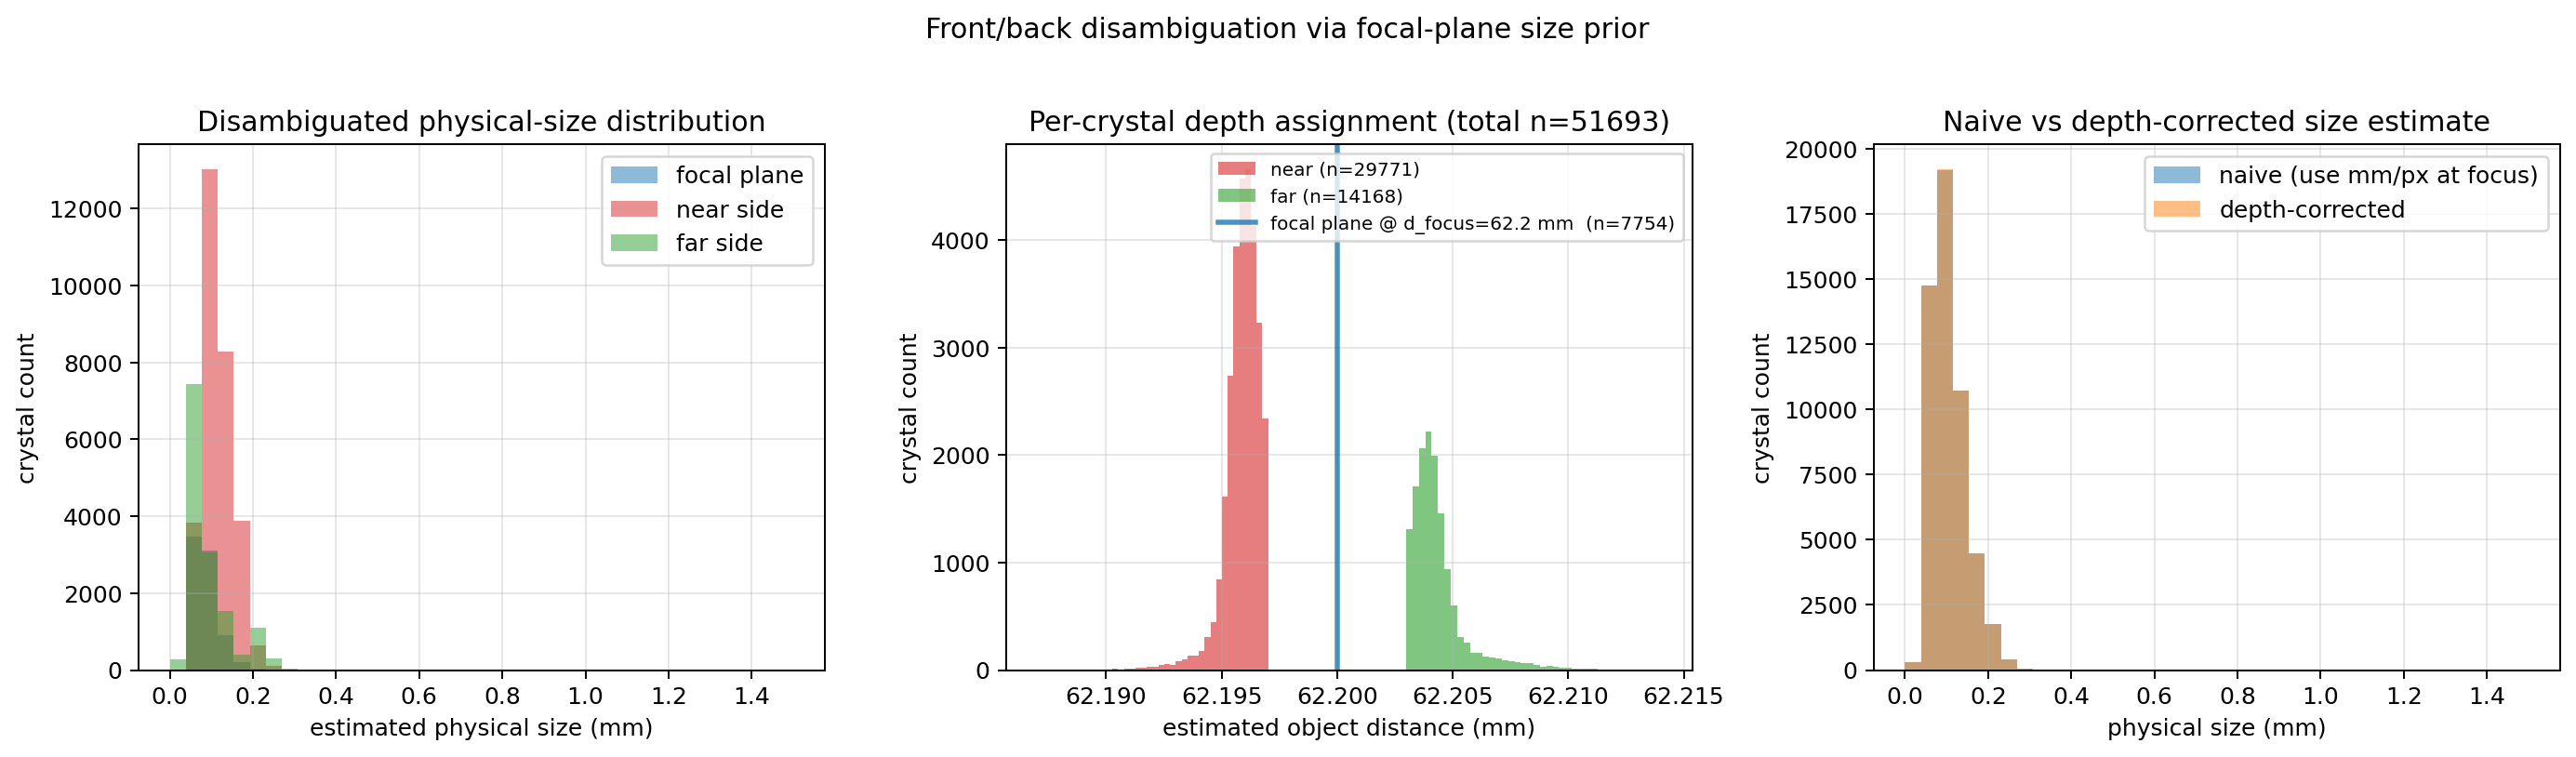
\includegraphics[width=\textwidth]{09_disambiguation}
\caption{Disambiguation output for the case-study clip (\texttt{optics.disambiguate}; watershed detector, configured
window, 52\,784 detections). Left: sizes by label. Middle: assigned depths; the near (33\,957) and far (10\,909)
clusters sit at 55.097 and 55.103~mm, a few micrometres either side of $d_\mathrm{focus} = 55.1$~mm, and 7\,918
detections form the focal subset. Right: sizes at $\Delta x(d_\mathrm{focus})$ and after depth correction; the two
histograms coincide. The near/far labels are tie-break outcomes (\secref{sec:disamb-result}).}\label{fig:disamb}
\end{figure*}

\subsection{Scale overlay at three assumed depths}\label{sec:overlay}

\figref{fig:overlays} draws a 0.1~mm grid and a 1~mm ruler on frame 750 at three assumed object distances. The clip
rows are resampled by 1.306 so that one displayed pixel is the same length on both axes and the grid is true in $x$
and $y$ (\code{scripts/rerun_paper_numbers.py --fig07}). Over $\pm 0.2$~mm the scale changes by $\pm 0.36$\,\%; the
window is 21 times the F/1.6 in-focus half-slice of $\pm 9.4$~\um{} (one PAL sample, \secref{sec:dof}). A single
scale at the focused plane is therefore adequate at this aperture. The sharpness map in the right panels is computed
from the image alone and is identical in all three panels; it shows which pixels carry sharp outlines, not their
depth.

\begin{figure*}
\centering
\begin{subfigure}{\textwidth}
\centering
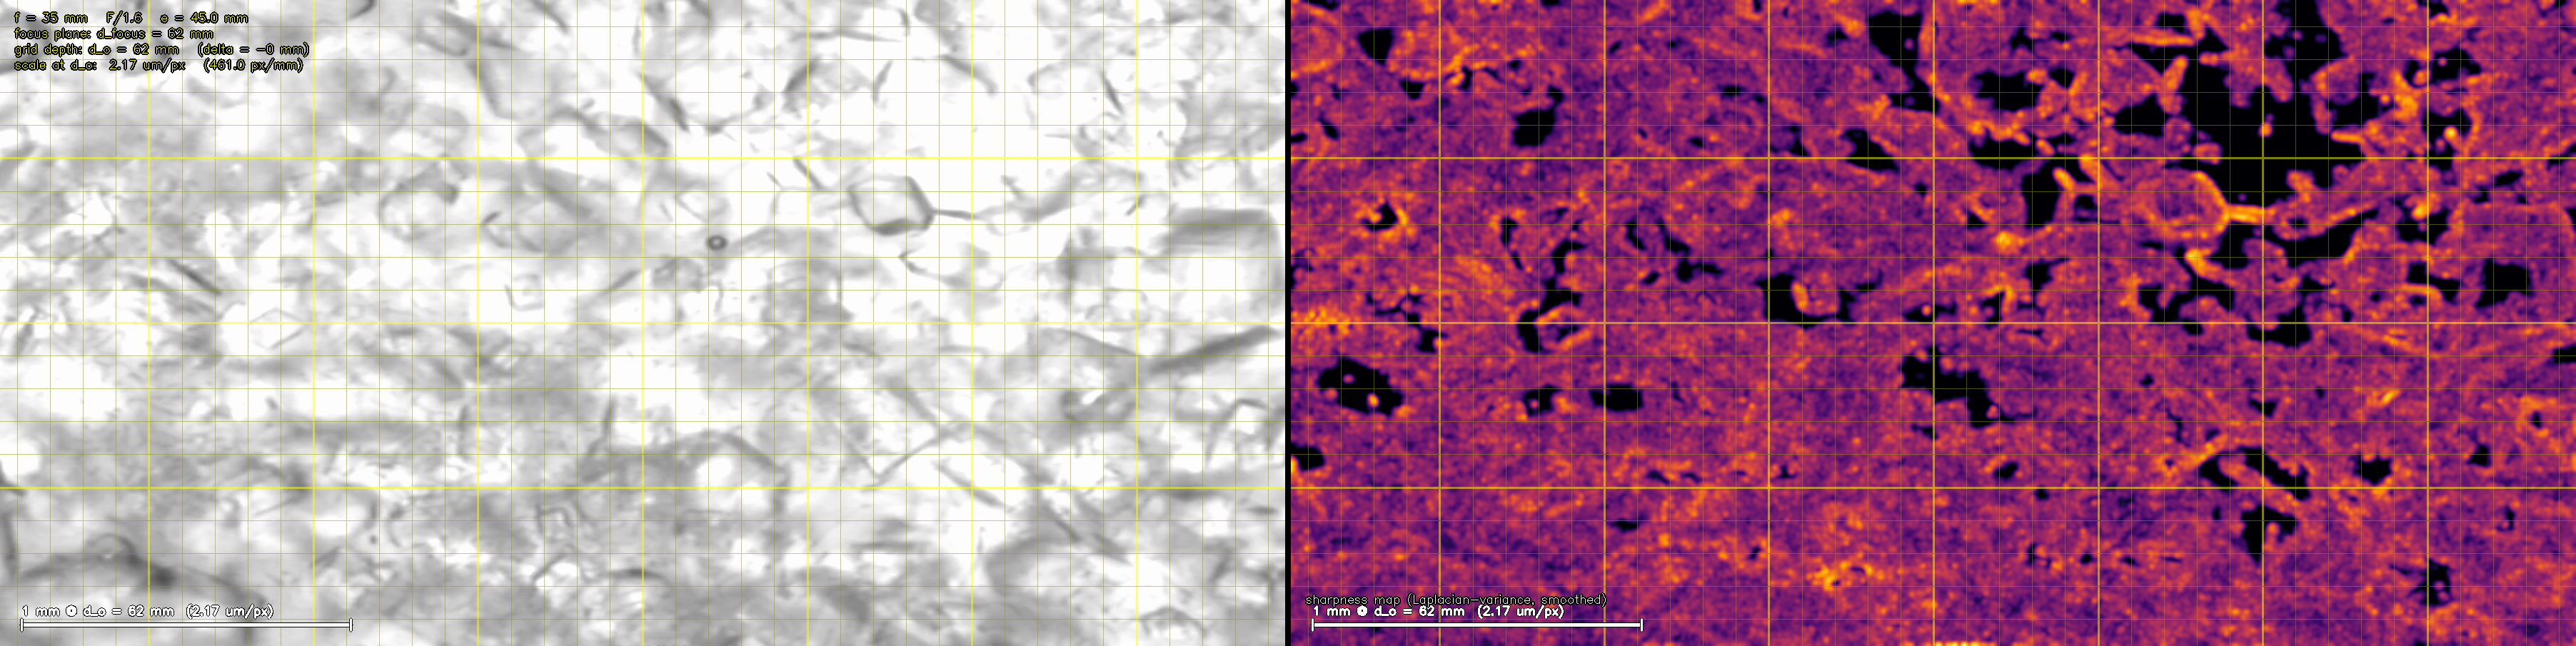
\includegraphics[width=0.8\textwidth]{07_overlay_near}
\caption{$d_o = 54.9$~mm: $1.460 \times 1.907$~\umpx{} ($x \times y$)}\label{fig:overlay-near}
\end{subfigure}

\medskip
\begin{subfigure}{\textwidth}
\centering
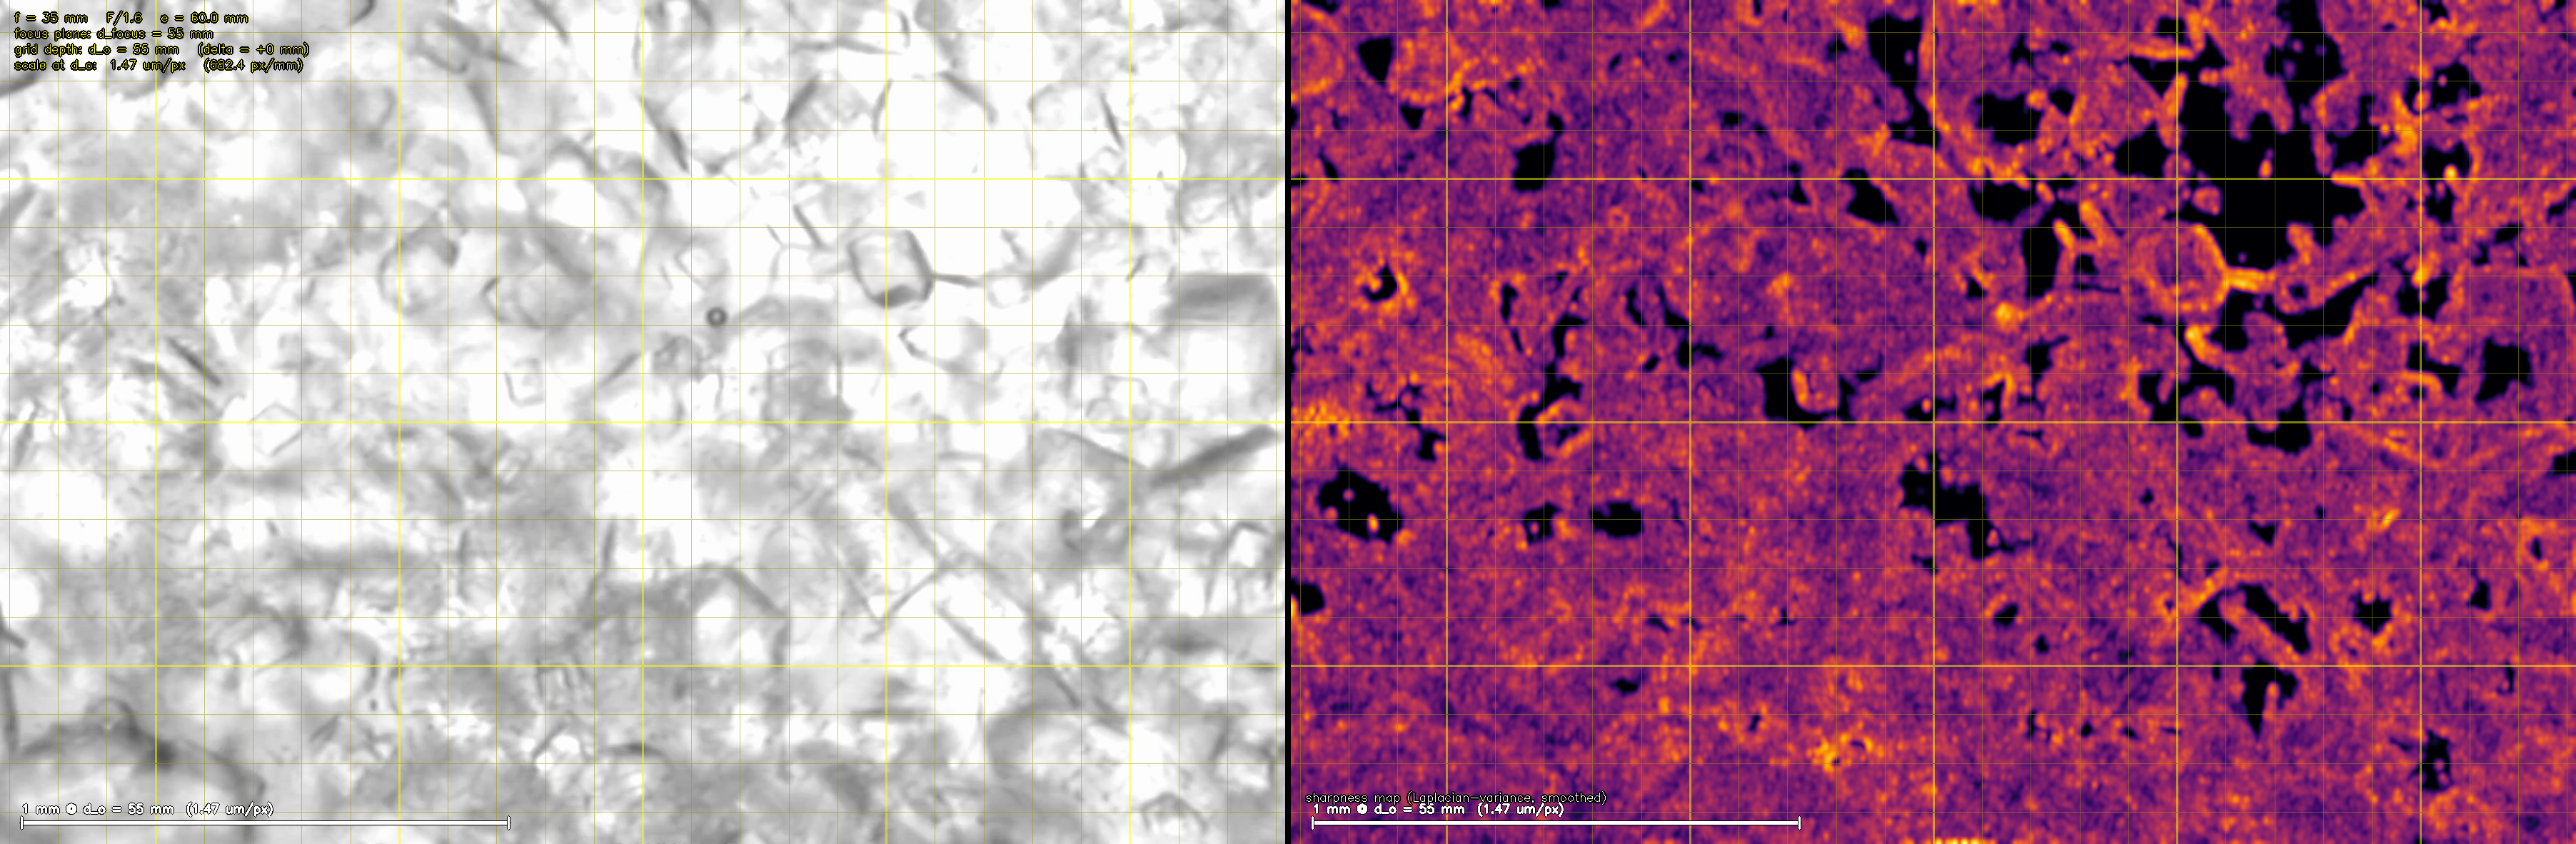
\includegraphics[width=0.8\textwidth]{07_overlay_at_focus}
\caption{$d_o = 55.1$~mm (focus): $1.465 \times 1.914$~\umpx}\label{fig:overlay-focus}
\end{subfigure}

\medskip
\begin{subfigure}{\textwidth}
\centering
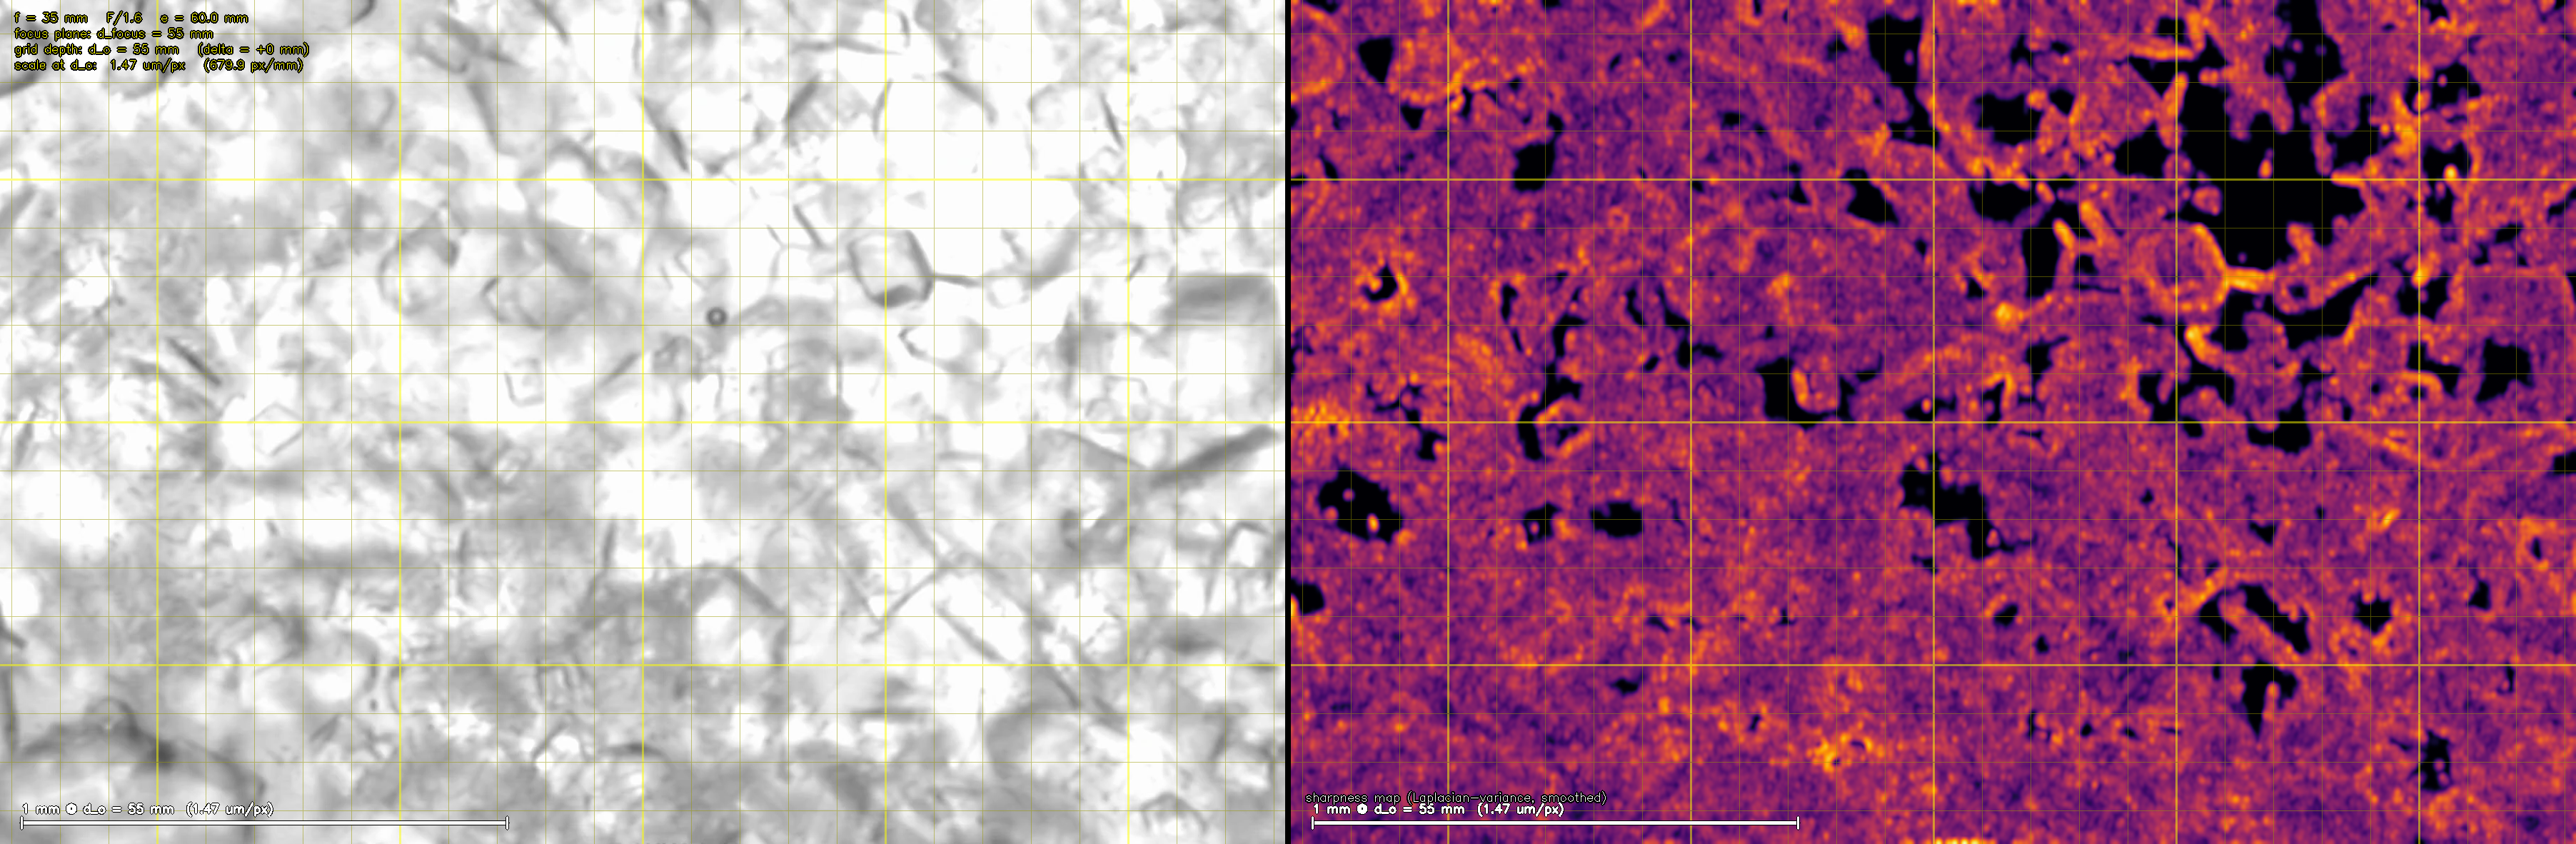
\includegraphics[width=0.8\textwidth]{07_overlay_far}
\caption{$d_o = 55.3$~mm: $1.471 \times 1.921$~\umpx}\label{fig:overlay-far}
\end{subfigure}
\caption{Scale grid (0.1~mm) and 1~mm ruler on frame 750 at three assumed object distances, with the rows resampled
so that the grid is true on both axes. Left: frame; right: sharpness map with the same grid. The scales in the
sub-captions are per clip pixel before resampling (ESTIMATE, $\pm\,{\approx}10$\,\% at 95\,\%); the on-image text
gives the resampled 1.47~\umpx{} and rounds $d_o$ to whole millimetres.}\label{fig:overlays}
\end{figure*}
